\paragraph{Example 1}{
\begin{lstlisting}[language=Python]
from BNumMet.NonLinear import IQI
fun = lambda x: x**2 - 2
points = [1, 1.5 ,2]
sol, nIter = IQI(fun, points, iters = True)
print("IQI method: x = %f, nIter = %d" % (sol, nIter))

>> IQI method: x = 1.414214, nIter = 6
\end{lstlisting}
}
\paragraph{Example 2}{
\begin{lstlisting}[language=Python]
from BNumMet.NonLinear import IQI
f = lambda x: sp.jv(0, x)  # Bessel function of the first kind of order 0
interval = lambda n: [
    n * np.pi,
    (((n + 1) * np.pi) - n * np.pi) / 2,
    (n + 1) * np.pi,
]  # Interval for the n-th zero

zeros = [IQI(f, interval(n)) for n in range(0, 7)]


x = np.arange(1, 10 * np.pi, np.pi / 50)
y = f(x)
plt.plot(x, y)
plt.plot(zeros, np.zeros(len(zeros)), "ro")
plt.axhline(0, color="k")
plt.title("Zeros of $J_0(x)$ with IQI method")
plt.xlabel("$x$")
plt.ylabel("$J_0(x)$")
plt.show()
\end{lstlisting}

\begin{figure}[H]
    \centering
    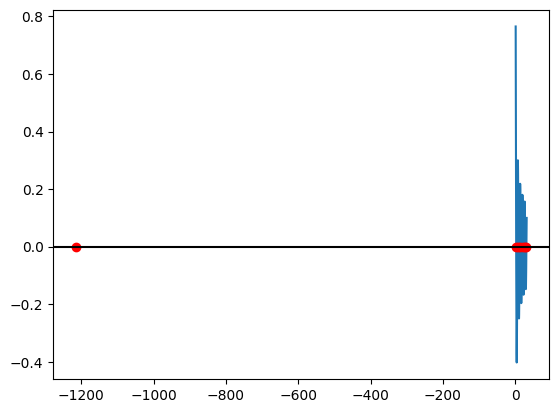
\includegraphics{Include/Images/Thesis/Documentation/NonLinear/IQI Example 2.png}
    \caption{IQI Example 2}
    \label{fig:IQI Example 2}
\end{figure}
}